\documentclass[conference]{IEEEtran}

\usepackage{cite}
\usepackage{amsmath,amssymb,amsfonts}
\usepackage{algorithmic}
\usepackage{graphicx}
\usepackage{ragged2e}
\usepackage{textcomp}
\usepackage[hyphens]{url}
\usepackage{xcolor}

\newcommand{\etal}{\textit{et al}. }

\def\BibTeX{{\rm B\kern-.05em{\sc i\kern-.025em b}\kern-.08em
    T\kern-.1667em\lower.7ex\hbox{E}\kern-.125emX}}

\begin{document}

\title{An Overview of Android Operating System Security}

\author{\IEEEauthorblockN{Kyler Dickey}
\IEEEauthorblockA{\textit{College of Engineering and Computer Science} \\
\textit{Arkansas State University}\\
Jonesboro, Arkansas, USA \\
kyler.dickey@smail.astate.edu}
}

\maketitle

\begin{abstract}
Android security is an imperative topic of discussion for researchers and developers due to its sheer scale on the market.
The platform is an appealing target for attackers because of the open nature of the platform's development, as well as the nature of the platform itself which attracts casual users that make use of the applications and services offered by the device to store sensitive and private information.
Android's security issues are made worse by inappropriate development practices, a lack of tools for those developers to adequately test and validate the security of their software, and the fragmentation of the platform.
A large portion of the vulnerabilities that exist in the Android platform are derived from low-level software components of the stack due to the pitfalls of low-level programming.
Significant research and attention have been given to the platform in the past decade, which is helping shore up the defenses of the platform to make the security components in the platform more robust and comprehensive.
\end{abstract}

\begin{IEEEkeywords}
Android Malware,
Android Vulnerabilities,
Mobile Platform Security,
Systems Security,
Privacy
\end{IEEEkeywords}

\section{Introduction}
The Android operating system (OS) is a mobile computing platform designed for personal use.
The OS platform is built on the Linux kernel and has additional components that facilitate application development and hardware interfacing \cite{AndroidDocs2022Arch}.
The platform is an open source project licensed under the Apache License \cite{Gilski2015}.

The platform consists of a number of layers referred to as the "software stack".
The lowest layer is the Linux kernel, on which the rest of the operating system components are built.
The next lowest layer is the hardware abstraction layer (HAL), which exists as an interface for hardware vendors to implement to ensure their hardware is compatible with the higher level components of the stack.
The next layer is the native libraries installed on the platform, which consist of widely-used low-level implementations of common services used by applications (encryption, rendering, etc.) provided for developer convenience as well as OS functionality.
The framework layer exists in the abstraction level above the native libraries and contains wrapper APIs for direct interfacing with a number of them.
The applications for the platform are built using the tools listed prior.
The Android runtime is also worth mentioning (the runtime exists at the same level of abstraction as the native libraries) because it ensures that applications run in their own virtual environment.

The Android platform has been maturing for well over a decade now, and has been reported to have a significant number of vulnerabilities in that time \cite{LinaresVasquez2017, Wu2019}.
Vulnerabilities seem to exist mostly in the Linux kernel layer and withing the supported native libraries.
The reason for this is likely due to the difficult nature of programming using low-level languages.

Android's worldwide market share is immense \cite{AndroidMarketShare2021}, which is likely what paints the platform as a lucrative target for attackers.
DroidKungFu, a particularly sophisticated malware family that targeted Android, exposed the platform at the time of its discovery outed the platform as woefully unprepared to deal with the threat of zero-day malware attacks, even from variants of known malware families \cite{Zhou2012}.
Since then, a significant amount of research attention has been given to the platform, especially within the domain of malware detection and prevention \cite{Faruki2015, Bhat2020}.

Android applications also suffer from a number of security issues.
Frequently, applications are implemented with incorrect protocols or applications contain misused components.
These cases of misuse introduce vulnerabilities into the applications that uses said protocols and components \cite{Qin2020, Zhan2021, Maalouf2021}.
Misuse of these components seems to stem partially from misunderstandings on the part of the developer.

Tools to help developers avoid programmatic pitfalls are constantly being developed.
Such tools would help programmers avoid introducing security issues into the applications made available to their user base and to the Android platform as a whole.
Examples of new tools that developers could use to secure the system include newer, safer programming languages and software designed to detect and mitigate vulnerabilities and malware that were developed through research.

This survey is partitioned into three sections.
Section I is a brief overview of the survey.
Section II is further divided into subsections.
Each subsection describes a part of the Android software stack and describes key vulnerabilities that exist at that layer.
Section III describes various malware-related vulnerabilities that exist or existed in the Android platform.
A discussion about the efficacy of malware detection on the platform is also specified.
Section IV describes other vulnerabilities in the Android platform that don't fit neatly anywhere else in the survey.
Section V concludes the survey and reaffirms courses of action that may be taken to increase the overall security of the platform.


\section{Android Architecture Security}
This section details the overall architecture of the Android OS and various security concerns at each level.
The operating system is composed of five major layers that facilitate access to the hardware components and software services provided by the OS.
Figure \ref{fig:AndroidArch} shows Android's architecture model by layer and is pulled directly from the Android developer documentation \cite{AndroidDocs2022Arch}.

\begin{figure}[htbp]
    \centerline{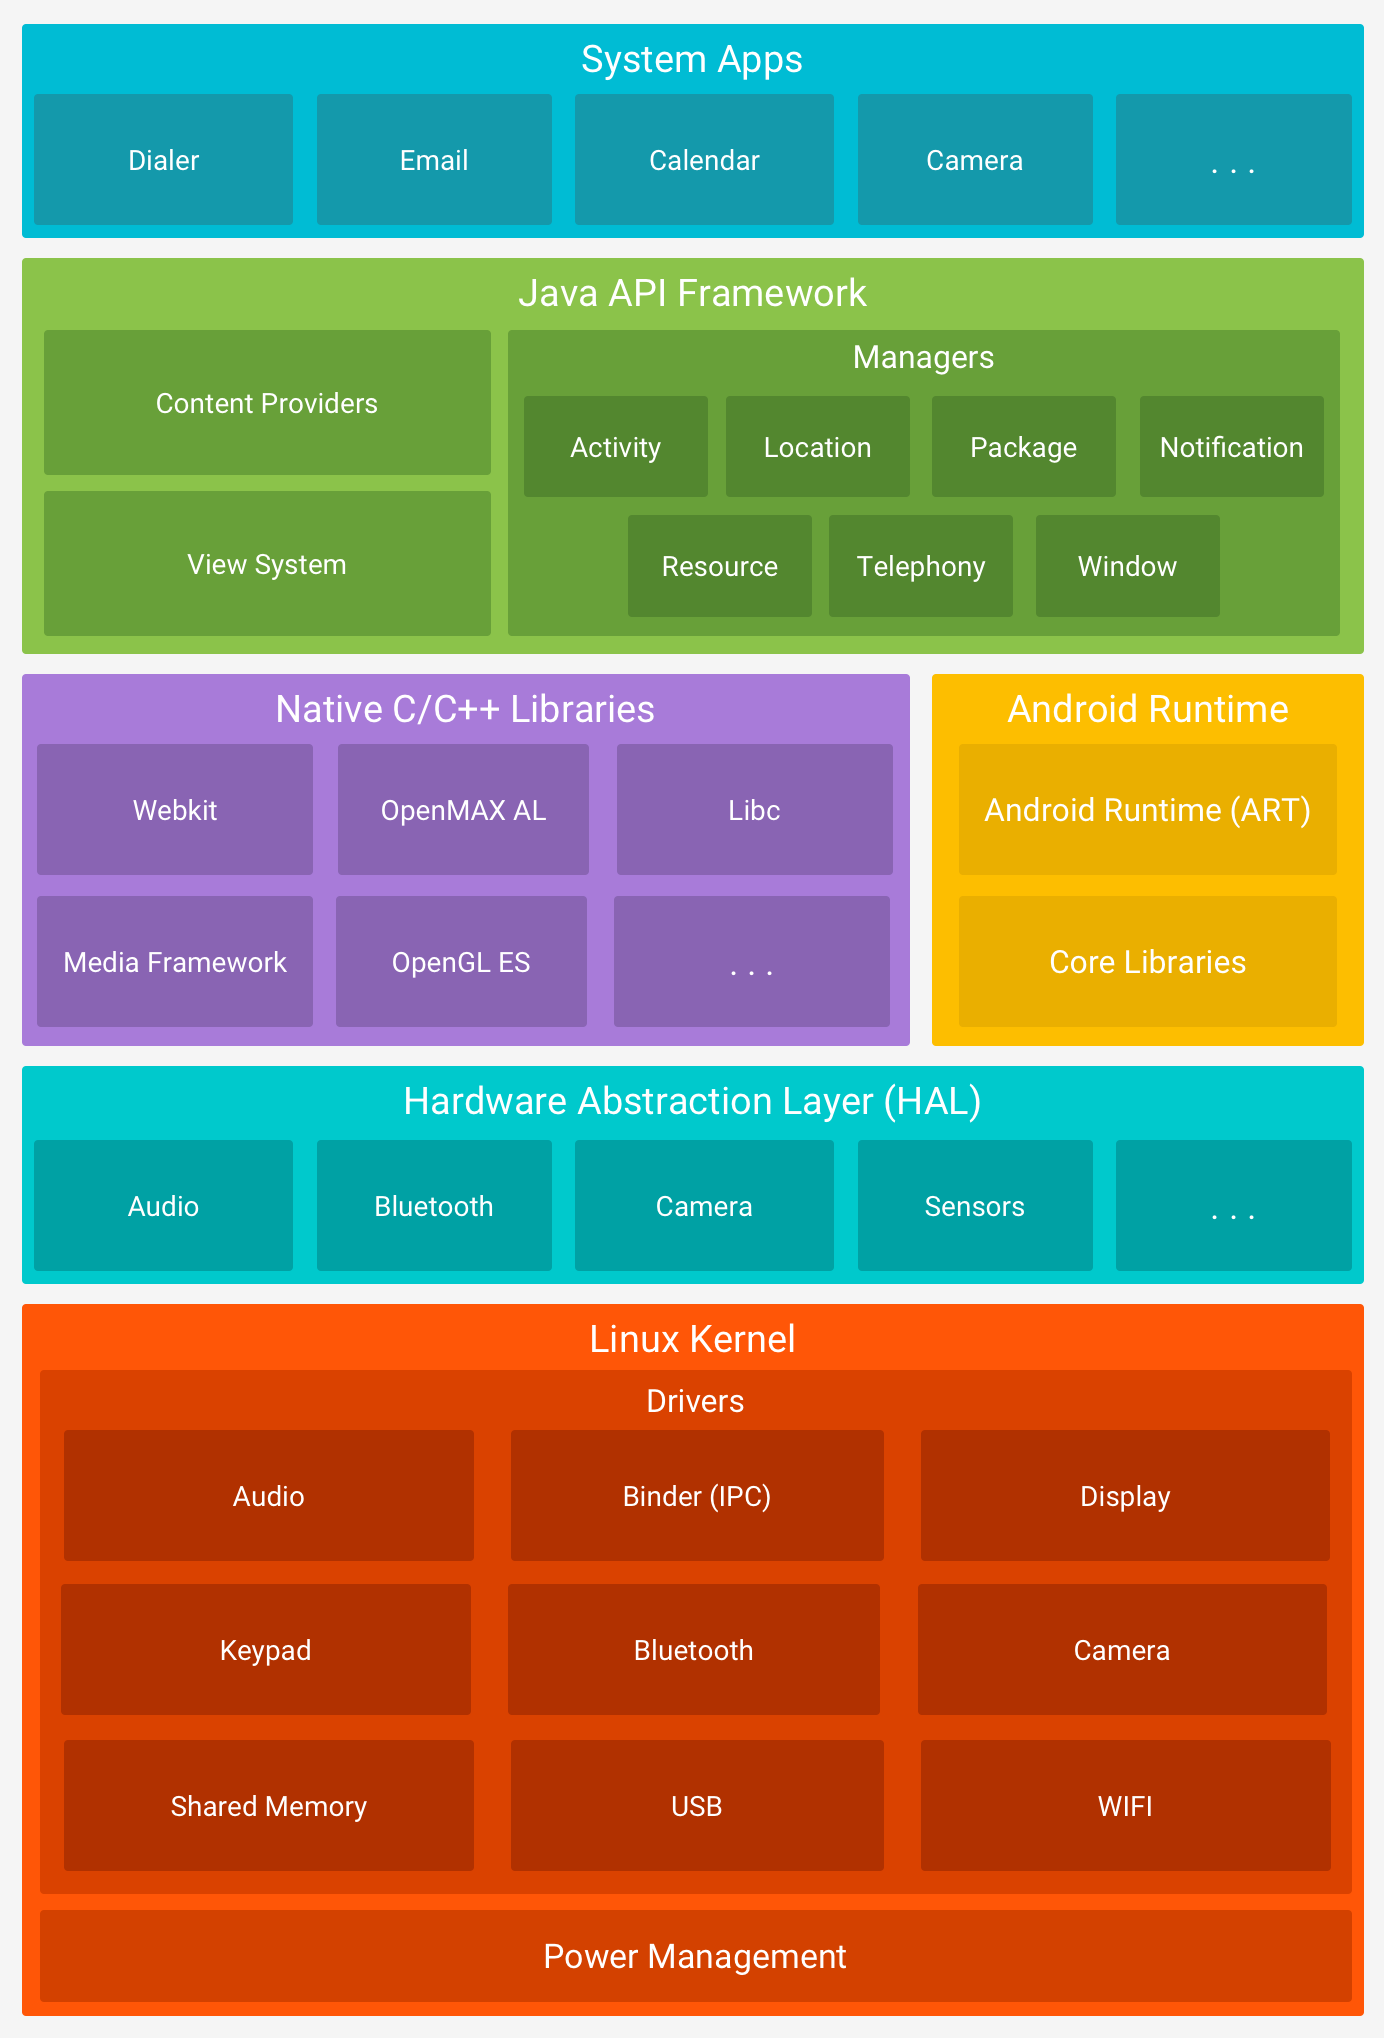
\includegraphics[width=0.4\textwidth]{figures/AndroidArch.png}}
    \caption{Android architecture model.}
    \label{fig:AndroidArch}
\end{figure}

Linares-Vasquez \etal breaks downs the vulnerabilities affecting the Android system \cite{LinaresVasquez2017}.
A majority of vulnerabilities occur at the lowest level of abstraction for the Android architecture model: the Linux kernel layer.
The next highest share of vulnerabilities exist within the native libraries supported by the Android platform.
These two portions of the Android architecture account for roughly 73\% of the sampled vulnerabilities studied.
This study provides a good overview of the distribution of vulnerabilities that exist in the Android platform.

\subsection{The Linux Kernel Layer}
The lowest part of the architecture stack is the Linux kernel that Android derived from.
The primary benefit of building an OS based on a Linux kernel is the maintenance performed on the Linux kernel by Linux developers.
In the case of Android, the overwhelming majority of bug fixes (95\%) are the result of work done by the Linux kernel development team \cite{Khomh2012}.

Another benefit of basing an OS on the Linux kernel is the wide range of functional OS support provided by the kernel already.
The adapted version of the Linux kernel used as the foundation to build the Android OS employs preexisting kernel features.
Most changes made to the Linux kernel adapted for Android extend current kernel functions or employ new features that make the OS more suitable for use on mobile devices, such as a more aggressive memory manager used to preserve the limited memory resources on the device and a power manager \cite{AndroidDocs2022Arch, Khomh2012}.

Linux kernel development, at the time of version 2.6, was carried out by a large group of developers from a multitude of different organizations and from developers acting independently \cite{KroahHartman2007}.
A significant portion of the kernel was dedicated to driver and architecture support, which is code that interfaces and provides hardware support.
This large pool of developers doesn't explicitly increase the safety of the software, since there is no substantial evidence to support the claim that open source software is more secure than a proprietary counterpart \cite{Schryen2009, Witten2001}.
Instead, the open source nature of the Linux kernel facilitates three key points:
\begin{itemize}
    \item Organizations may develop drivers for their own hardware and maintain a measure of control over their own hardware security as a result. More generally, users have direct control when improving security of open source systems.
    \item Organizations and their developers may trust open source software more than a proprietary alternative.
    \item Organizations and their developers gain access to new features of the kernel approved by the maintainers of the source code.
\end{itemize}

The last point is particularly pertinent.
The earliest versions of Android were based on the Linux kernel 2.6 versions \cite{Gilski2015}.
These versions of the Linux kernel introduced the Linux Security Modules (LSM), which is a framework for general purpose access control \cite{Wright2002}.
The LSM explicitly supports the implementation of different security models that already existed at the time the feature was introduced, without favoring one over the other.
A notable example would be SELinux, which is an extensive, non-discretionary access control implementation contracted by the National Security Agency (NSA) that was adapted to use the LSM \cite{Smalley2001}.
Access to these types of security feature updates are important for implementing OS functionality such as the mandatory access control that exists in more recent versions of the Android OS \cite{AndroidDocs2022SELinux}.

Third-party hardware drivers are the largest source of vulnerabilities within the kernel.
This means that hardware vendors introduce the highest amount of vulnerable code into the project \cite{LinaresVasquez2017}.
A possible reason for this is a vendor's profit incentive.
So long as the majority the consumers of the vendor's products believe that the amount of risk associated with owning a device with insecure drivers is acceptable, those consumers will continue to pay for the device.
A lack of interest or tangible change from the perspective of consumers that comes from security-related development gives a vendor no reason to deviate from the business model of developing the new features instead of securing existing systems \cite{Witten2001}.

\subsection{Hardware Abstraction Layer}
The HAL exists as an interface because the higher level application programmable interfaces (API) needs to remain the same for platform application developers \cite{AndroidDocs2022Arch}.
In order to decouple the kernel drivers from the higher layers, the concrete implementation of the HAL is left to the hardware vendors.
Only the vendor would have knowledge of the hardware used to assemble the device and the drivers used to control them.

Since the layer is an abstraction expected to be fulfilled by the aforementioned vendors, Android cannot explicitly trust the code inside concrete implementations as authentic.
However, the HAL is among the least affected layers when it comes to security-related vulnerabilities, according to the study done by Linares-Vasquez \etal \cite{LinaresVasquez2017}, meaning the vulnerabilities are less likely to exist in the HAL layer.
The largest sources of vulnerabilities within the layer in the sample used in the study are the media component interfaces.

\subsection{Android Runtime}
The Android Runtime, like the HAL, suffers very little from vulnerabilities in comparison to the other layers.
This layer consists of the Dalvik Virtual Machine (VM) or the Android runtime (ART) and the core runtime libraries that provide functionalities within the scope of the Java programming language \cite{JavaDocs2022}.
The Dalvik VM and the ART are the environments that the system applications and some system services run on \cite{AndroidDocs2022Arch}.

Most of the vulnerable code in this layer (of which there is comparatively low amount of compared to other parts of the Android software stack) exists in the core libraries.
Core libraries are derived from the implementations of the Java programming language.
Android has since moved to using OpenJDK \cite{OpenJDK2022} over other implementations, mainly due to legal issues between Google LLC and Oracle America Inc. over the latter's claim of copyright infringement \cite{Oyez2020, Amadeo2016}.

Bugs may exist in the implementations that provide attackers with information about a system.
These forms of attacks are called side-channel attacks \cite{Tiri2007}.
The behavior of an implementation, such as the time intervals of system calls and power consumption, can be observed by an attacker to glean information about the aforementioned implementation.
The attacker may then combine that information with knowledge about algorithms or standards used by the system.
For example, an attacker's knowledge of encryption algorithms may be combined with information extracted from a system implementation may allow the attacker to determine the value of a key.

Tizpaz-Niari \etal demonstrated a tool, FUCHSIA, developed to detect the presence of side channels \cite{TizpazNiari2018}.
In the study, the researchers found a zero-day side-channel vulnerability in OpenJDK implementation.
Early returns in a method used in the cryptography library resulted in code that could have been exploited by timing side-channel attacks.
This issue has since been resolved by the OpenJDK development team, but is a good example of the types of implementation vulnerabilities that have the potential to affect the Android platform core libraries.

\subsection{Native Libraries}
Native libraries in the Android platform consist of native compiled code that is specific to the system hardware architecture \cite{AndroidDocs2022Arch}.
These native libraries are typically implemented in C \cite{Kernighan1988} and/or C++ \cite{Stroustrup2013}.
The implementation of these libraries in low-level languages like C and C++ is important because low-level programming languages tend to offer better performance than other languages (namely Java, the primary language used for Android application development) in terms of computation time and memory usage \cite{Prechelt2000}.
Memory usage is particularly important for mobile embedded devices, since such devices tend to have limited capabilities for scaling the amount of physical memory that can be fitted onto the device.

Native libraries are utilized in the Android platform in two ways.
First, the native libraries are used by the Android system itself to implement low-level components such as those in the HAL.
Second, Android provides wrapper APIs written in Java for native libraries.
These wrapper APIs allow programmers to access some native libraries made available by the Android system without re-implementing them in Java (which wouldn't be an optimal use of the system's limited resources anyway).
This has the added benefit of reducing the amount of development maintenance needed to keep the hypothetical re-implementations patched.

A study done by Daoyuan Wu \etal further corroborates the findings in the study conducted by Linares-Vasquez \etal in regard to breaking down the ratio of vulnerabilities per layer of the Android platform \cite{LinaresVasquez2017, Wu2019}.
Both studies report that the native libraries own the second-highest number of vulnerabilities, with the Linux kernel having the absolute highest number of vulnerabilities in both cases as well.
Both studies also report that a large portion of the vulnerabilities that exist in the native library layer is due to poor handling of memory allocated by the libraries, especially by media and communication components.

The most likely reason for the sheer quantity of vulnerabilities in both the Linux kernel layer and the native library layer lies in the code.
Both layers are largely implemented in low level programming languages.
It is far more difficult to write secure code in C and C++ especially because of the lack of any safety features that exist in languages like Java, which has robust bounds checking on data structures \cite{JavaDocs2022}.
These safety features come at the cost of reduced performance, but greatly reduce the chance of a program being exploitable since a program written in a language with bounds checking will raise an exception or error instead of allowing the program to continue unchecked.

Poor memory handling has the potential to be catastrophic for any computerized system.
Vulnerabilities like the buffer overflow open the floodgates for a multitude of different attacks, let alone accidental memory corruption.
There are numerous examples of the different attacks that may be conducted from buffer overflow vulnerabilities \cite{Lhee2003, Kuperman2005}.

\begin{figure}[htbp]
    \centerline{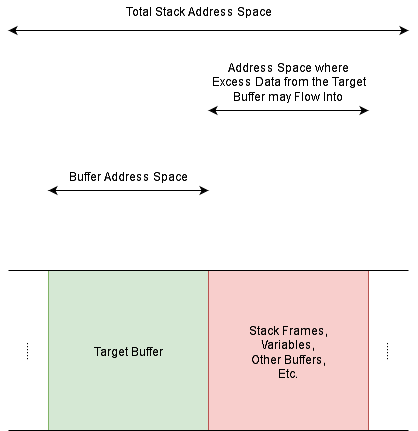
\includegraphics[width=0.4\textwidth]{figures/BufferOverflow.png}}
    \caption{High-level diagram of a buffer overflow.}
    \label{fig:BufferOverflow}
\end{figure}

Figure \ref{fig:BufferOverflow} is a high-level abstraction of a buffer overflow in memory.
It should be noted that the buffer overflow can overwrite parts of a stack frame.
Attackers can intentionally overwrite the return address of the stack frame to redirect a program to malicious code.

One such example of an attack conducted via buffer overflow is an attack on Android's KeyStore service \cite{Hay2014}.
The KeyStore service allows the user to securely store keys for cryptographic operations \cite{AndroidDocs2022Keystore}.
Keys are stored on disk in files containing key as ciphertext (keys are stored in encrypted form).
The keys are identified by filename.
The lack of bounds checking on buffers present in the code (explicitly left out by the KeyStore authors for performance reasons) allows a programmer to inject arbitrary data into the stack memory through the Java API.
By using exploiting this vulnerability, an attacker could inject malicious code that could leak the unencrypted keys.
This attack is particularly damaging to a user, since the keys stored in the KeyStore could be used by applications installed on the device to access sensitive information.

It is difficult to overstate the importance of detecting and patching memory-related vulnerabilities.
Since both the Linux kernel and the native library layers of the Android platform make use of low level languages that tend to allow these vulnerabilities, attacks may be conducted from a multitude of places within the software stack.
Savvy attackers with a robust knowledge of a system's inner workings may find and exploit the vulnerabilities found from reviewing source code.
At the same time, white hat hackers and researchers may also review the code and find vulnerabilities in the code and notify the maintainers so that the code may be patched.
This is the double-edged sword of open source software.

In the meantime, researchers are developing tools to assist in the detection and prevention of memory corruption.
A long-term solution might include the development of more modern, safer programming languages that avoid the classic pitfalls that come with programming applications and libraries in C and C++.
One such example is the Rust programming language, which prevents unsafe memory operations at compile time unless explicitly told to ignore them using the "unsafe" keyword built into the language \cite{Rust2022}.
The "unsafe" keyword has the added benefit of making the code searchable if the aforementioned unsafe operations ultimately do result in exploitable or buggy code.

Other solutions might be the complete isolation of native libraries into a non-privileged environment, as proposed by Sun and Tan \cite{Sun2014}.
Their model proposes the loading of native code into a separate application all on its own that has only the permissions it needs to perform its functions (principle of least privilege).
This limits the scope of the memory the native code has access to, decreasing the threat of memory corruption.
This is an improvement, since normally native code has full access to a device's memory.
It is clear, though, that there is no catch-all solution to fully patch and prevent these exploits in the native libraries (and in the Linux kernel).

\subsection{Application Framework Layer}
The application framework layer consists of a Java API that allows a programmer to access the services provided by the Android platform \cite{AndroidDocs2022Arch}.
Both Linares-Vasquez \etal and Wu \etal report several vulnerabilities in the Activity Manager that exists at this layer \cite{LinaresVasquez2017, Wu2019}.
The activity manager is a service that oversees the application that are actively running on the system.

Armando \etal describe a Denial-of-Service (DoS) attack carried out by Android's Activity Manager \cite{Armando2012}.
The DoS attack effectively creates a fork bomb, filling the device memory space with identical processes until an automatic device reboot is triggered (which would cause an infinite boot loop in the case of the program being run from the bootloader).
The attack exploits the mechanisms through which Android creates new processes via the Activity Manager, which involves interoperating with the Linux kernel layer to create new processes.

Attacks on the Activity manager are a good example of the types of vulnerabilities that may exist in the application framework layer.
Such attacks highlight a particularly unsafe part of the framework, since vulnerabilities here could potentially cause a loss of availability to one or many applications or services.
Other areas of interest might be the telephony API, the built-in web browser, or any other component that facilitates communications and connections (which tend to be vulnerable to man-in-the-middle attacks among others).

\subsection{Application Layer}
The application layer is where the programs accessible by the end user of the device exist.
These applications range from short messaging service (SMS) applications, to web browsers, to calculators.
Applications are allowed to use each other's services in order to reduce the burden on the programmer to provide code for features users would want from an application (such as two-factor authentication, autofill from a password manager, etc.) \cite{AndroidDocs2022Arch}.
Application security in the Android environment is discussed at length in Section IV.


\section{Android Malware}
Android malware poses a significant threat to the user base of the platform.
Smartphones are a vital tool for many and functions as a platform for work and play.
Android, being a leader in the smartphone OS market worldwide, is used by a significant number of people \cite{AndroidMarketShare2021}.
The safety of this platform is of critical importance to ensure that the users of the OS do not incur personal losses and to ensure that the platform may not be a medium for larger scale attacks on networks.

Recalling earlier discussion about the application framework layer in the Android platform \cite{AndroidDocs2022Arch}, it is clear that a large collection of powerful tools are available to the programmer.
Furthermore, it is possible to download and install applications not listed on any app stores as long as those applications fulfill the application requirements and follow the APK format \cite{AndroidDocs2022Fundamentals}
These conditions (powerful, easy to use, well documented platform software tools and an attack surface with little to no moderation) make Android a ripe target for Trojans, adware, and otherwise potentially unwanted applications (PUAs).

In a study published in 2012 about the characterization of malware targeting the Android platform, Zhou and Jiang reported that 86.0\% of the malware sample they characterized were repackaged applications containing malicious code that was added by the attackers \cite{Zhou2012}.
Furthermore, the study highlights an outbreak of a notorious Android malware named DroidKungFu.
The outbreak of DroidKungFu included the initial version of the malware, as well as several version iterations and variants.

As DroidKungFu evolved through variants and versions, it became more sophisticated.
For example, the malware inside a repackaged application could install a functional copy of the malware payload onto the device.
This ensured that the malware would remain even if a user uninstalled the original infected program from the device.
This payload was encrypted in later versions.
Encryption is a sophisticated obfuscation technique used by attackers to hide their malware.

In fact, in the same study that publicized the existence of DroidKungFu, Zhou and Jiang found that mobile antivirus services were inadequate solutions to malware detection \cite{Zhou2012}.
The software used to detect malware on the platform seemed to struggle to detect newer versions of the same malware family, due to the latter's rapid evolution and the former's use of signature-based detection.

Signature-based malware detection is considered to be largely ineffective when defending against so called "zero-day" malware, which is a fancy term for unmitigated operational malware that exists on live system, sometimes without the user's knowledge.
Signature-based malware detection schemes rely on pre-existing knowledge of a malware's existence, since a signature needs to be generated against the malware.
This gives zero-day malware time to propagate, damage, leak data, and otherwise cause harm to the platform ecosystem \cite{You2010}.

The fact that malware like DroidKungFu circumvented the techniques used by antivirus services through versioning and branching variants is a topic of concern.
It is apparent that malware authors only need to expend minimal effort to obfuscate their malware.
In the case of DroidKungFu, the release of newer versions might have only taken a matter of months.

Faruki \etal give a good overview of the types of malware that threaten the Android platform, as well as other vulnerabilities and issues with the system (which is discussed in Section IV) \cite{Faruki2015}.
This survey also highlights a number of efforts that have been made to secure the platform against threats and study them.
The study also provides a robust and clear breakdown of a number of malware families and the timeline of their emergence.


\section{Other Android Security Challenges}
One of the principal reasons that the Android platform suffers from a plethora of security issues is fragmentation \cite{Zhou2014, Gilski2015, Faruki2015}.
The fragmentation of the Android platform is derived from the various customizations new devices undergo during development.
Customizations may include hardware drivers and pre-installed applications.
As stated prior, the hardware drivers that exist in the Android platform are a significant source of vulnerabilities.

Since the implications and mechanics of the vulnerabilities at the low-level parts of the stack have been discussed at length in Section II, the main focus of this section will be on the applications.
A study done by Zhou \etal discusses the security implications of Android's fragmentation issue \cite{Zhou2014}.
In the study, the researchers found that the topic was not well researched and that different images of the Android OS customized by hardware vendors contained security vulnerabilities.
Particularly, a number of apps that came pre-installed on some images were given excessive privileges, among other issues.

In regard to responsible application development, Android applications are not always up to an acceptable standard.
Web applications are a large source of vulnerabilities, which opens them up to network-based attacks.
Third party libraries (code libraries written to assist in application development with the goal of reducing the burden of implementing complicated or repetitive aspects of other programs) are also a common source of vulnerabilities.
The reason for these vulnerabilities seems to be, in large part, by developers who are either unaware of the potential vulnerabilities of their system, a lack of awareness or domain knowledge of the components used in their system, or a lack of understanding for how to use a particular technology \cite{Qin2020, Zhan2021}.

One domain of misuse includes OAuth implementations. OAuth is an open standard for access control mechanisms built into Internet services.
A common use case is to use the standard in an application to access the information of a service from another service or application if user permission is given.
A study conducted by Wang \etal found that applications vendored by both American (specifically the Google Play Store) and Chinese Android app markets demonstrated misuse of the OAuth protocol \cite{Wang2015}.
Part of the reason for this seemed to be a lack of understanding of the specifications by the developers.
Figure \ref{fig:OAuth2Oracle}, sourced from Oracle's documentation \cite{OAuth2ControlOracle}, demonstrates a typical control flow for the OAuth 2.0 protocol.

\begin{figure}[htbp]
    \centerline{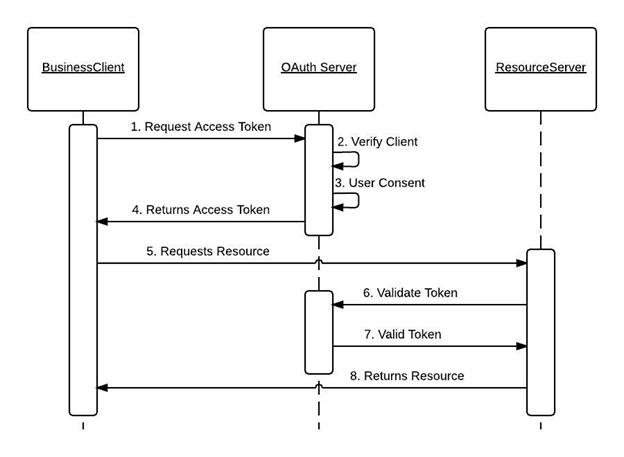
\includegraphics[width=0.5\textwidth]{figures/OAuth2Oracle.png}}
    \caption{OAuth 2.0 protocol control flow.}
    \label{fig:OAuth2Oracle}
\end{figure}

Another misuse case may be derived from a native library supported by the Android platform: SQLite \cite{SQLite}.
SQLite is a widely used embeddable SQL relational database engine.
SQLite, like other SQL databases, is susceptible to query injection \cite{Maalouf2021}.

Expanding on SQLite some more, a peculiar quirk that sets it apart from other SQL databases is access control.
SQLite effectively have no access control mechanisms because the file is stored on disk (access to that file may be controlled like any other, but it does not extend to the tables, columns, rows, etc. stored in the file).
Mutti \etal propose an SELinux-like model to the SQLite database included in the Android platform to improve access control to databases stored on-device \cite{Mutti2015}.
Since applications on Android are sandboxed and are assigned their own user identifier, permissions could be given to certain applications to access only the subset of the database it needs, allowing applications to exchange data securely.

Application development on the Android platform could be significantly improved with the invention of tools that assist in the testing and verification of code safety.
Developers could find themselves under significant time pressure, might be using unfamiliar components or standards, or may engage in happy-path testing.
Programmers could produce poor quality code for any number of reasons.
Tools and automation are consistent when developing sensitive systems and may help reduce the human aspect of flawed software.


\section{Conclusion}
A multitude of vulnerabilities have existed in every part of the Android platform.
In particular, the platform suffers from common pitfalls encountered when a system is implemented using low-level programming languages like C and C++.
These low level components exist in the Linux kernel layer and the native library layer in the platform's software stack.
In the kernel layer, most of the vulnerabilities tend to come from hardware vendors implementing drivers for their products.
In the native library layer, most vulnerabilities are derived from media-related libraries.

Malware is a pervasive threat to the Android platform, DroidKungFu being a particularly sophisticated example.
Malware, left untreated and undetected, may do significant harm to users of the platform.
Fortunately, new developments and research projects are being conducted on an ever-growing scale to combat the issue.

Other security concerns mainly pertain to inappropriate programming practices and lack of developer tools to ensure the deployment of robust code.
Examples of this concern include SQL injections on the native SQLite library included in the Android platform as well as misused authentication protocols.
Table \ref{tab:AndoridPlatVuln} lists the various vulnerabilities that affect each layer of the Android software stack.

Steps may be taken to reduce the effect these vulnerabilities, such as updating the libraries to use modern languages with safeguards against exploitable memory errors and using compiler tools to detect faults before runtime.
Work could be done to provide developers with tools to bolster the security of their systems by that could be used to detect, correct, and code to decrease number of vulnerabilities in the low-level systems.
Adoption of better development practices and tools would drastically improve Android's current security situation going forward.
However, fixing issues on existing systems would prove exceptionally challenging.
The intense fragmentation of the platform exacerbates the issue of security by scattering the number of Android versions available on the market, making it difficult to manage and preventing some users from receiving important updates.

The Android platform is used on a large scale worldwide, and is seen as a lucrative target by attackers because of its sheer scale.
As a result, the security of the system should be ensured by the developers and maintainers of the software used to build the platform, from the Linux kernel to the application framework.
Furthermore, maintainers of reputable application sources should constantly take steps to ensure their reputability by keeping their platform free of malicious applications that could cause damage to users.

\begin{table*}[tbp]
    \normalsize
    \centering
    \caption{Android Platform Vulnerabilities}
    \label{tab:AndoridPlatVuln}
    \begin{tabular}{p{0.25\linewidth}p{0.7\linewidth}}
    \hline
    \hline
    Software Platform Layer    & Vulnerability Examples Directly Affecting the Platform Layer                                                \\ \hline
    Linux Kernel               & Corrupted Bootloader, Buffer Overflow, Data Leaks, Insecure Driver Code, Malicious Code Injection, Rootkits \\
    Hardware Abstraction Layer & Untrustworthy Code Written by Third Party Vendors                                                           \\
    Native Libraries           & Buffer Overflow, Malicious Code Injection                                                                   \\
    Android Runtime            & Side-Channel Attacks on Core Libraries                                                                      \\
    API Framework              & Built-In Web Browser Abuse, DoS Attacks via the Activity Manager, Telephony API Misuse                      \\
    Applications               & Absence of Database Security, Adware, Authentication Protocol Misuse, Inappropriate Permissions, Trojans    \\
    \hline
    \hline
    \end{tabular}
\end{table*}


\begingroup
\raggedright
\setlength{\emergencystretch}{3em}
\bibliographystyle{IEEEtran}
\bibliography{IEEEFull}
\endgroup

\end{document}
